% !TeX spellcheck = fr_FR
\chapter{Chapitre 4 : Lignes et appariement par lignes}

\noindent Ce chapitre propose une visite guidée de la couche \emph{lignes} : comment nous construisons une vue unifiée des lignes à partir de GTFS et HRDF, à quoi ressemblent les données, ce que disent les chiffres, et comment nous effectuons l'appariement basé sur les lignes entre les arrêts ATLAS et les nœuds OSM.

\section{Des flux bruts à un fichier unique de lignes}
\subsection{Ce qu'est \texttt{atlas\_routes\_unified.csv}}
Nous consolidons les \emph{signaux de ligne} issus de deux sources dans un seul fichier tabulaire :
\begin{itemize}
  \item \textbf{GTFS} : identifiants de ligne, noms court/long, et la direction (0/1). Les directions sont dérivées via une heuristique \emph{premier$\rightarrow$dernier} par trajet, agrégée au niveau de la ligne.
  \item \textbf{HRDF} : noms de lignes et chaînes de direction construites comme \emph{première gare$\rightarrow$dernière gare}, à la fois par noms et par paires de codes UIC.
\end{itemize}
Chaque ligne du CSV décrit « un signal de ligne pour un arrêt » :

\begin{table}[H]
\caption{Structure du fichier \texttt{atlas\_routes\_unified.csv}}
\label{tab:atlas_routes_unified}
\centering
\small
\begin{tabular}{|l|p{8cm}|}
\hline
Colonne & Signification \\
\hline
\texttt{sloid} & Identifiant d'arrêt ATLAS\\
\hline
\texttt{source} & \texttt{gtfs} ou \texttt{hrdf}\\
\hline
\texttt{evidence} & Méthode d'inférence (p. ex. \texttt{gtfs\_first\_last}, \texttt{hrdf\_fplan})\\
\hline
\texttt{as\_of} & Date d'extraction\\
\hline
\texttt{route\_id}, \texttt{route\_id\_normalized} & ID GTFS brut et normalisé par année\\
\hline
\texttt{route\_name\_short}, \texttt{route\_name\_long} & Noms de ligne GTFS\\
\hline
\texttt{line\_name} & Ligne HRDF (si disponible)\\
\hline
\texttt{direction\_id} & Direction GTFS 0/1 (chaîne)\\
\hline
\texttt{direction\_name}, \texttt{direction\_uic} & Chaînes premier$\rightarrow$dernier\\
& humaines et UIC\\
\hline
\end{tabular}
\end{table}
Cette structure est produite directement par l'écriture unifiée. La \textbf{normalisation par année} supprime les suffixes saisonniers (p. ex. \texttt{-j24}) pour stabiliser la comparaison entre les années :

\begin{codebox}[language=Python]{Normalisation des identifiants de ligne}
import re
def normalize_route_id(route_id: str) -> str:
    return re.sub(r"-j\\d+", "-jXX", route_id)
\end{codebox}

\subsection{Comment on le génère (vue d'ensemble)}
Le processus de haut niveau (voir \texttt{get\_atlas\_data.py}) est le suivant :
\begin{enumerate}
  \item Charger GTFS en flux et ne garder que les arrêts suisses (IDs commençant par \texttt{85}).
  \item Premier passage sur \texttt{stop\_times} : pour chaque \texttt{trip\_id}, collecter le premier et le dernier arrêt suisses ; joindre à \texttt{trips} et \texttt{routes} pour obtenir l'ID et les noms de ligne.
  \item Construire, par ligne, les chaînes de direction « nom du premier arrêt $\rightarrow$ nom du dernier arrêt » (dédupliquées).
  \item Second passage sur \texttt{stop\_times} : dédupliquer \((\texttt{stop\_id},\ \texttt{route\_id},\ \texttt{direction\_id})\).
  \item Mapper \texttt{stop\_id} GTFS vers \texttt{sloid} ATLAS (règle stricte puis repli sûr).
  \item Parser HRDF (\texttt{GLEISE\_LV95}, \texttt{FPLAN}, \texttt{BAHNHOF}) pour obtenir lignes et directions premier$\rightarrow$dernier par \texttt{sloid}.
  \item Écrire un unique CSV propre combinant les deux sources.
\end{enumerate}

\section{Ce que disent les données unifiées}
Les chiffres ci-dessous sont calculés avec les scripts sous \texttt{memoire/scripts\_used/chap4}.

\subsection*{Vue GTFS}
\begin{itemize}
  \item \textbf{SLOIDs avec lignes GTFS} : \textbf{34\,781}
  \item \textbf{Nombre moyen de lignes uniques par \texttt{sloid}} : \textbf{2,73} (médiane \textbf{2,00})
  \item \textbf{Nombre moyen de couples (ligne, direction) par \texttt{sloid}} : \textbf{4,39} (médiane \textbf{3,00})
  \item \textbf{Taux de duplication pour (\texttt{sloid}, route\_norm, direction)} : \textbf{96,96\%}
  \item \textbf{Même ligne+direction, plusieurs chaînes de direction} : \textbf{96,95\%} des groupes présentent plus d'une chaîne premier$\rightarrow$dernier (ce qui indique des schémas d'exploitation hétérogènes).
\end{itemize}

\subsection*{Vue HRDF}
\begin{itemize}
  \item \textbf{SLOIDs avec lignes HRDF} : \textbf{28\,757}
  \item \textbf{Nombre moyen de lignes uniques par \texttt{sloid}} : \textbf{2,32} (médiane \textbf{2,00})
  \item \textbf{Directions distinctes par (\texttt{sloid}, line\_name)} : \textbf{2,67} par UIC et \textbf{2,67} par nom (médianes \textbf{2,00})
  \item \textbf{Longue traîne} : plusieurs couples (\texttt{sloid}, ligne) affichent \textbf{30--40} paires UIC premier$\rightarrow$dernier distinctes (branches, demi-tours)
\end{itemize}

\paragraph{En résumé.} \emph{GTFS} couvre un grand nombre d'arrêts avec plusieurs directions par ligne ; \emph{HRDF} confirme une forte variété de directions terminales pour certaines lignes (longue traîne). Cela implique qu'une comparaison robuste doit gérer la multiplicité des directions, et pas seulement les identifiants de ligne.

\begin{figure}[H]
  \centering
  \begin{minipage}[b]{0.48\textwidth}
    \centering
    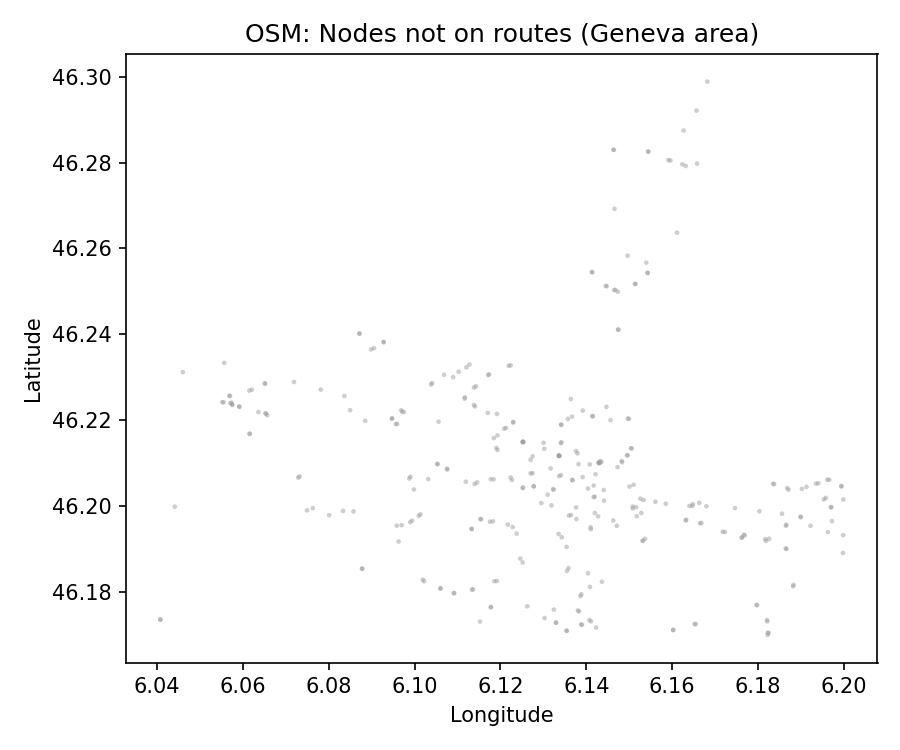
\includegraphics[width=\textwidth]{../figures/chap4/geneva_osm_non_routes_nodes.png}
    \caption*{OSM : nœuds ne faisant partie d'\emph{aucune} relation de ligne (Genève).}
  \end{minipage}\hfill
  \begin{minipage}[b]{0.48\textwidth}
    \centering
    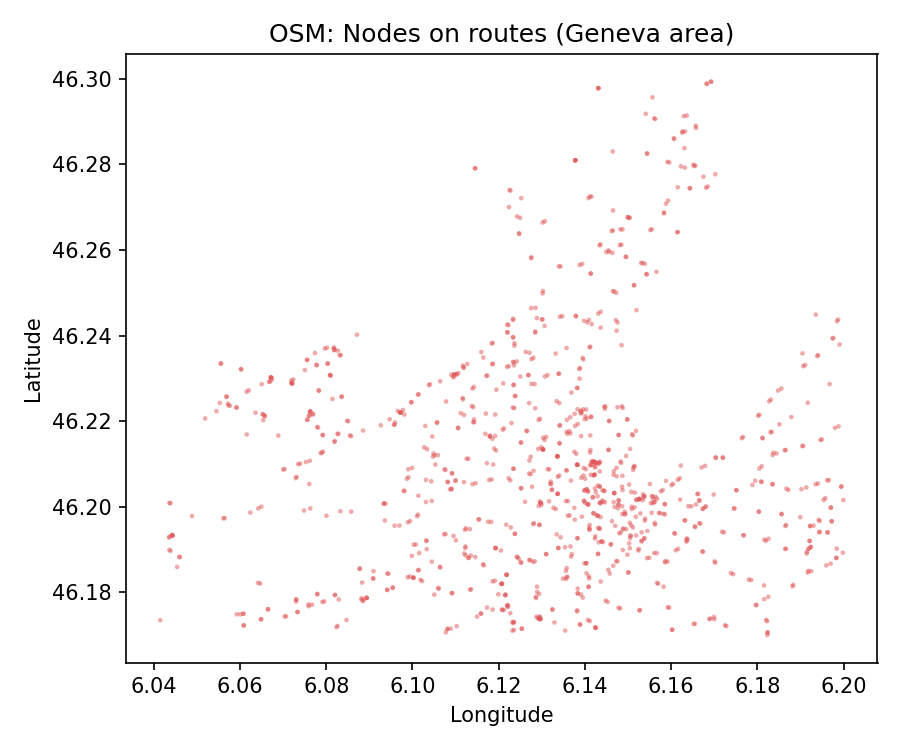
\includegraphics[width=\textwidth]{../figures/chap4/geneva_osm_routes_nodes.png}
    \caption*{OSM : nœuds participant à \emph{au moins une} relation de ligne (Genève).}
  \end{minipage}
  \caption{Nœuds OSM hors lignes vs. sur des lignes (région de Genève).}
\end{figure}

\begin{figure}[H]
  \centering
  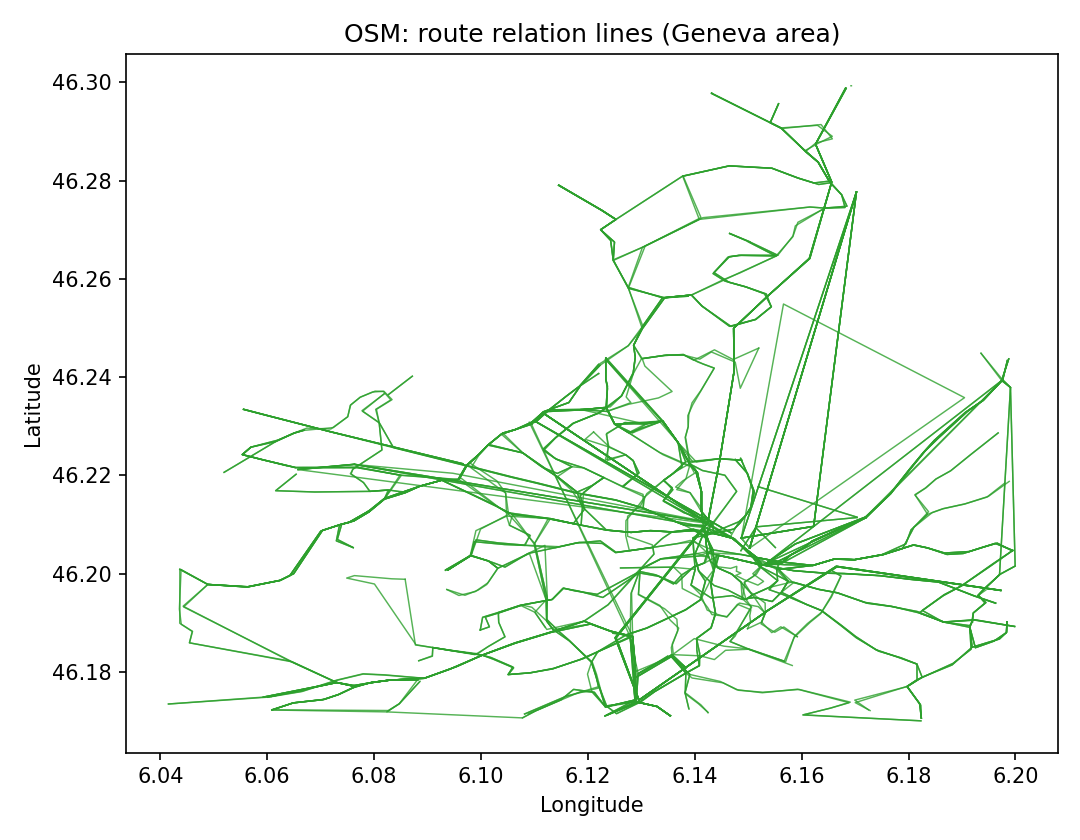
\includegraphics[width=0.8\textwidth]{../figures/chap4/geneva_osm_route_lines.png}
  \caption{OSM : tracé des lignes à partir des relations de type \texttt{route} (Genève). Géométrie bien structurée.}
\end{figure}

\begin{figure}[H]
  \centering
  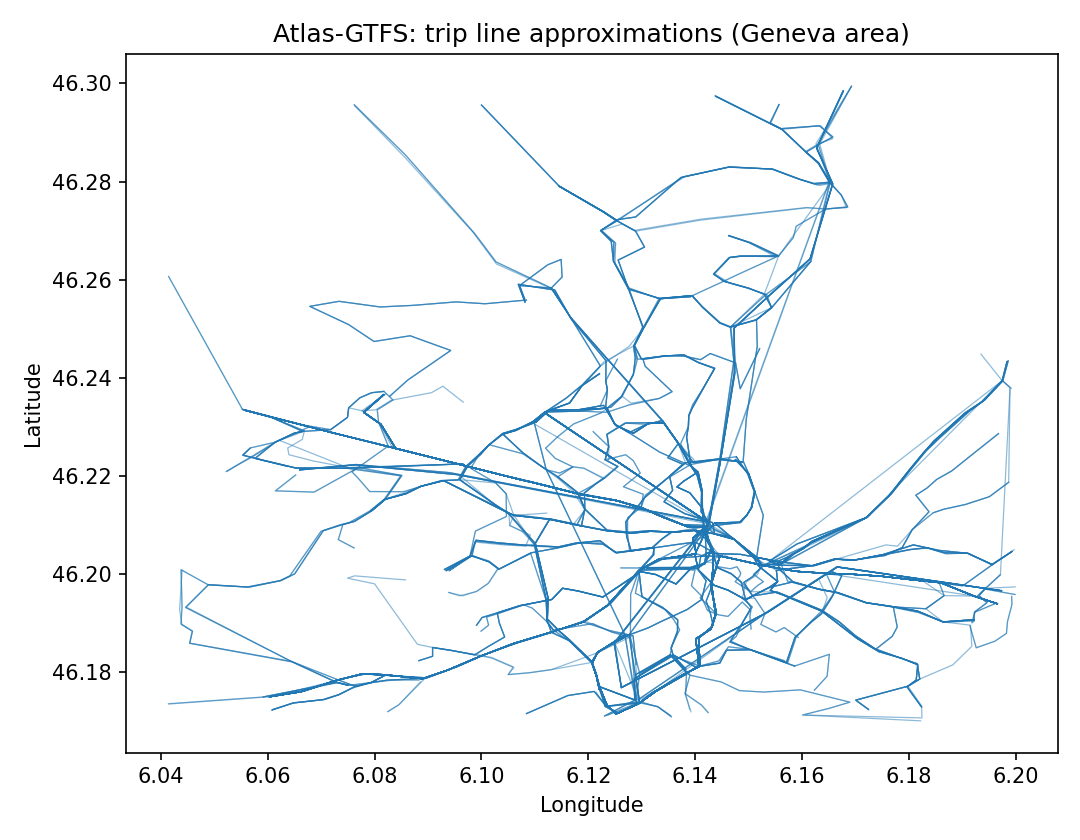
\includegraphics[width=0.8\textwidth]{../figures/chap4/geneva_atlas_gtfs_trip_lines.png}
  \caption{Atlas-GTFS : approximation des trajets (Genève). Lignes reconstruites depuis l'ordre des arrêts — plus fragmenté.}
\end{figure}

\begin{codebox}[language=Python]{Tracer les lignes \emph{Atlas-GTFS} (simplifié)}
stops = read_csv('stops.txt')[['stop_id','stop_lat','stop_lon']]
stop_times = read_csv('stop_times.txt')[['trip_id','stop_id','stop_sequence']]

# 1) Restreindre aux arrêts dans la boîte Genève
stops_ge = stops[in_bbox(stop_lat, stop_lon)]
stop_times_ge = stop_times[stop_id \in stops_ge.stop_id]

# 2) Reconstituer les séquences ordonnées par trajet
seq_map = {tid: tuple(g.sort_values('stop_sequence').stop_id)
           for tid, g in stop_times_ge.groupby('trip_id') if len(g) >= 2}

# 3) Compter les séquences répétées et en échantillonner
seq_counts = Counter(seq_map.values())
chosen = choose_top_sequences(seq_counts, max_trips=500)

# 4) Projeter en coordonnées et tracer
for seq in chosen:
    pts = [stops_ge.loc[id][('stop_lat','stop_lon')] for id in seq]
    draw_polyline(filter_in_bbox(pts))
\end{codebox}

\section{D'autres vues utiles}
\begin{figure}[H]
  \centering
  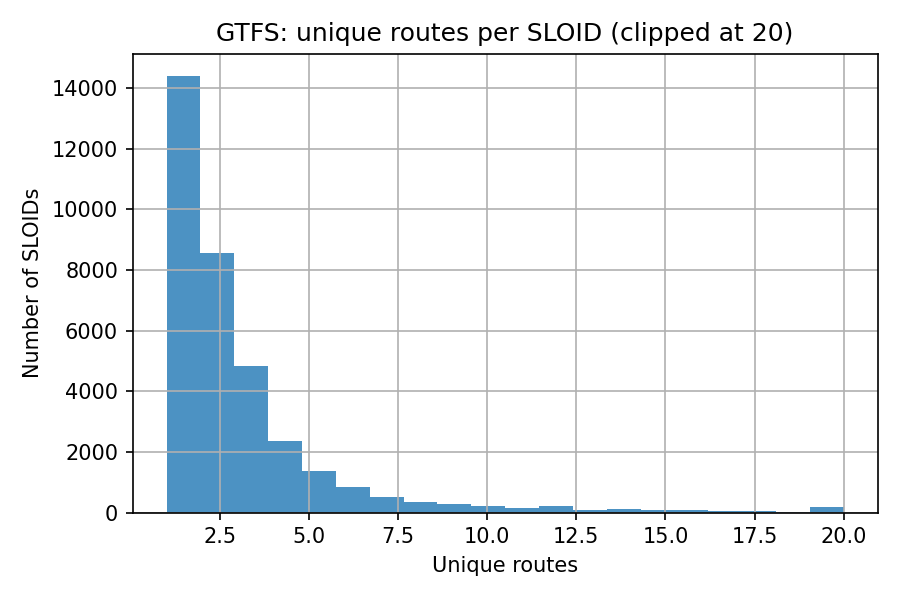
\includegraphics[width=0.75\textwidth]{../figures/chap4/hist_gtfs_routes_per_sloid.png}
  \caption{Distribution du nombre de lignes GTFS uniques par \texttt{sloid} (coupée à 20).}
\end{figure}

\begin{figure}[H]
  \centering
  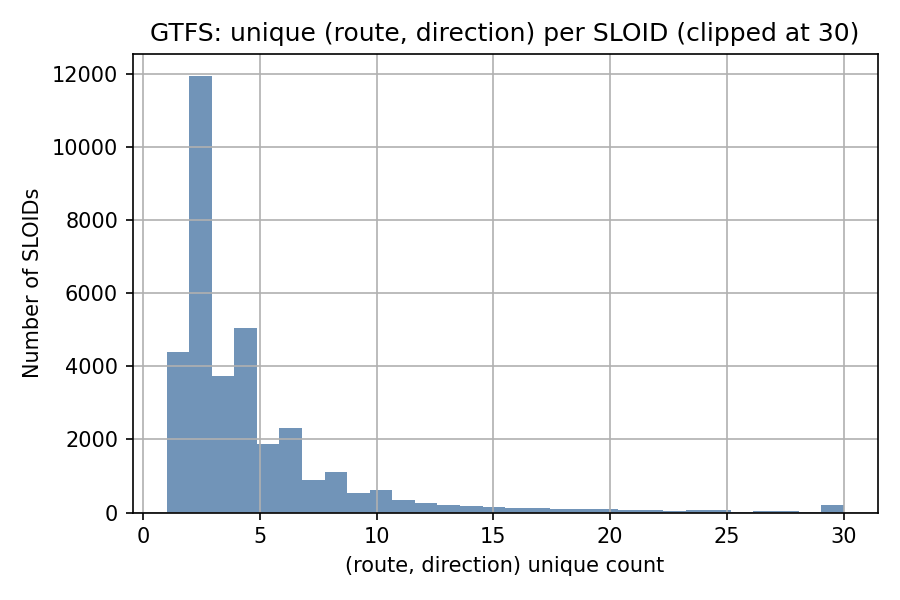
\includegraphics[width=0.75\textwidth]{../figures/chap4/hist_gtfs_route_dir_per_sloid.png}
  \caption{Distribution du nombre de couples (ligne, direction) par \texttt{sloid} (coupée à 30).}
\end{figure}

\begin{figure}[H]
  \centering
  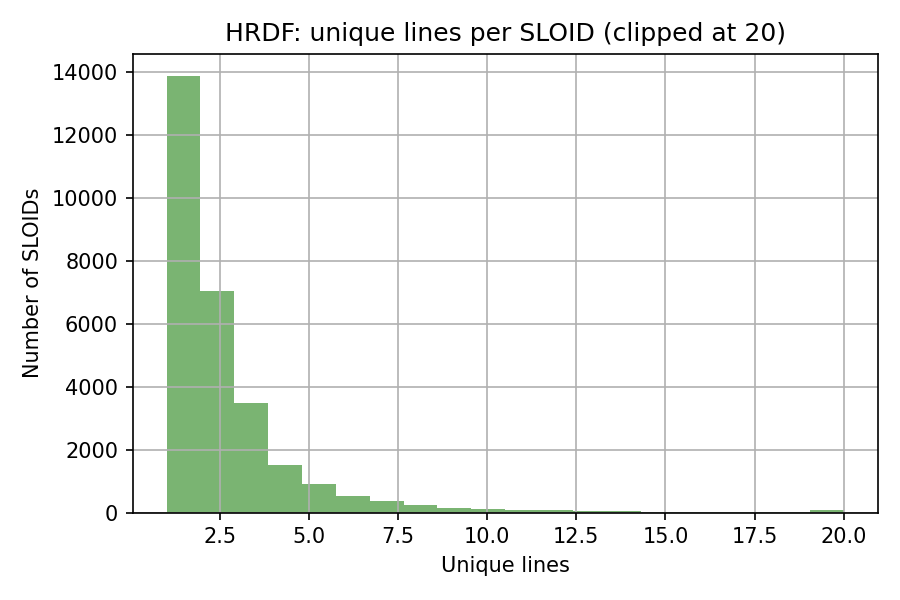
\includegraphics[width=0.75\textwidth]{../figures/chap4/hist_hrdf_lines_per_sloid.png}
  \caption{Distribution du nombre de lignes HRDF uniques par \texttt{sloid} (coupee a 20).}
\end{figure}


\begin{itemize}
  \item \textbf{GTFS --- lignes par \texttt{sloid}} : moyenne \textbf{2,733}, mediane \textbf{2,0}, p10 \textbf{1}, p90 \textbf{5}, max \textbf{58}. \emph{Lecture} : la plupart des arrets ont 2--5 lignes, quelques hubs depassent largement.
  \item \textbf{GTFS --- (ligne, direction) par \texttt{sloid}} : moyenne \textbf{4,392}, mediane \textbf{3,0}, p10 \textbf{1}, p90 \textbf{8}, max \textbf{95}. \emph{Lecture} : les directions doublent naturellement la diversite par rapport aux seules lignes.
  \item \textbf{HRDF --- lignes par \texttt{sloid}} : moyenne \textbf{2,318}, mediane \textbf{2,0}, p10 \textbf{1}, p90 \textbf{4}, max \textbf{33}. \emph{Lecture} : structure comparable a GTFS, avec des extremes moins frequents.
\end{itemize}

\subsection*{Comment obtenons-nous les \emph{tokens} HRDF UIC ?}
Rappel synthétique de notre méthode (détaillée au Chapitre~1), qui s'appuie sur trois fichiers HRDF principaux pour extraire les informations de direction :
\begin{itemize}
    \item \textbf{\texttt{GLEISE\_LV95}} est d'abord utilisé pour lier chaque \texttt{sloid} de quai à l'UIC de sa gare et à une référence de quai locale (\texttt{\#ref}). Cela nous permet d'identifier tous les voyages desservant un quai spécifique.
    \item \textbf{\texttt{FPLAN}} est ensuite consulté pour les voyages pertinents afin de déterminer leur direction. Nous y extrayons le premier et le dernier arrêt de chaque trajet (sous forme de codes UIC), ainsi que le nom de la ligne.
    \item \textbf{\texttt{BAHNHOF}} fournit les noms de gares correspondant aux codes UIC, ce qui nous permet de construire des chaînes de direction lisibles (par exemple, \texttt{"Genève $\rightarrow$ Lausanne"}) ainsi que des chaînes basées sur les UIC (par exemple, \texttt{"8501008 $\rightarrow$ 8501120"}).
\end{itemize}
Ces tokens \((\texttt{line\_name},\ \texttt{direction\_uic})\) sont comparés aux chaînes UIC premier$\rightarrow$dernier dérivées d'OSM pour appuyer l'appariement au niveau HRDF lorsque les identifiants GTFS manquent dans OSM.

\section{Fonctionnement de l'appariement par lignes}
L'appariement compare les tokens de ligne connus pour un \texttt{sloid} ATLAS aux tokens dérivés des nœuds OSM à proximité (KD-tree, rayon configurable : \texttt{50 m} par défaut). Les tokens sont soit \textbf{GTFS} \((\texttt{route\_id},\ \texttt{direction\_id}), avec normalisation éventuelle\), soit \textbf{HRDF} \((\texttt{line\_name},\ \texttt{direction\_uic})\).

\subsection{Candidats par distance}
Nous tentons l'appariement en quatre paliers :
\begin{enumerate}
  \item \textbf{P1/P2 (tokens GTFS)} : intersection non vide entre les tokens GTFS du \texttt{sloid} et ceux d'un noeud candidat.
  \item \textbf{P3 (HRDF par UIC)} : presence d'une chaine UIC premier$\rightarrow$dernier du cote du noeud (membre d'une relation OSM) correspondant a une chaine HRDF du \texttt{sloid}.
  \item \textbf{P4 (repli par noms)} : concordance entre une chaine \emph{nominale} OSM premier$\rightarrow$dernier et une chaine unifiee (cote ATLAS).
\end{enumerate}
Extrait minimaliste de la logique des tokens :

\begin{codebox}[language=Python]{Intersection de tokens GTFS}
node_tokens = set()
for route in node_routes:
    rid = route.gtfs_route_id
    did = route.direction_id or '0'
    if rid:
        node_tokens.add((rid, did))
        rid_norm = normalize_route_id(rid)  # '-j25' -> '-jXX'
        if rid_norm:
            node_tokens.add((rid_norm, did))

if gtfs_tokens & node_tokens:
    match = ('gtfs', 'gtfs_tokens')
\end{codebox}

La normalisation des identifiants de ligne utilisée dans tout le système est :

\begin{codebox}[language=Python]{Normalisation \texttt{route\_id}}
import re

def normalize_route_id(route_id: str) -> str:
    return re.sub(r"-j\\d+", "-jXX", route_id)
\end{codebox}

\subsection{Paramètres}
\begin{itemize}
  \item \textbf{Rayon} : \texttt{50 m} par défaut. Plus petit $\Rightarrow$ moins de faux positifs, mais risque de manquer des arrêts légèrement décalés dans OSM.
  \item \textbf{Types de tokens} : activer uniquement GTFS ou inclure les paliers HRDF.
  \item \textbf{Normalisation} : comparer avec ou sans \texttt{-jXX}.
\end{itemize}

\section{Résultats de l'appariement par lignes}
\begin{itemize}
  \item \textbf{Tokens GTFS} : \texttt{7\,252} ; \textbf{tokens OSM} : \texttt{7\,121} ; \textbf{chevauchement} : \texttt{3\,200} ; \textbf{Jaccard} : \textbf{0,2864}.
  \item \textbf{Couverture par \texttt{sloid} (GTFS)} : moyenne \textbf{2,64}, médiane \textbf{2}, p90 \textbf{6} ; au moins un token couvert pour \textbf{73,4\%} des \texttt{sloid}s.
  \item \textbf{Au niveau des lignes} : lignes GTFS uniques \textbf{3\,839} ; avec correspondance OSM \textbf{1\,664} $\rightarrow$ \textbf{43,3\%} de lignes appariées.
  \item \textbf{Chaînes UIC premier$\rightarrow$dernier} : HRDF \textbf{8\,818}, OSM \textbf{5\,633}, chevauchement \textbf{2\,935}.
\end{itemize}
\noindent \emph{Interprétation} : la similarité \textbf{Jaccard $\approx 0{,}29$} indique un recouvrement substantiel mais non total des tokens GTFS dans OSM ; le taux d'appariement \textbf{43\%} au niveau des lignes confirme une couverture utile pour un appariement de haute précision.

\paragraph{Illustration de la similarité de Jaccard.} Rappel : \(J(A,B) = \frac{|A \cap B|}{|A \cup B|}\). Ci-dessous, deux vues complémentaires — un histogramme des tailles et un schéma par cercles — pour contextualiser les ordres de grandeur.

\begin{figure}[H]
  \centering
  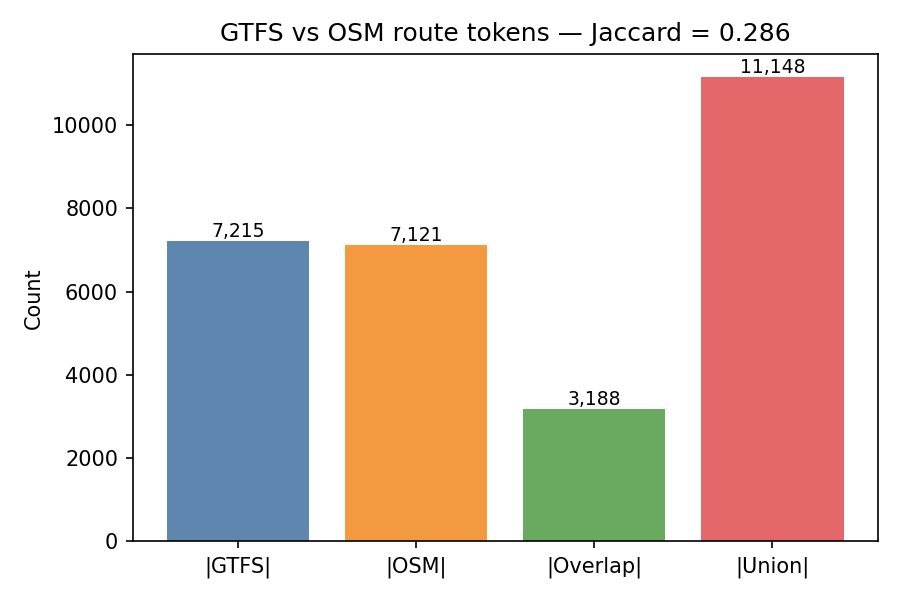
\includegraphics[width=\textwidth]{../figures/chap4/jaccard_sets_bars.png}
  \caption*{Tailles \(|\mathrm{GTFS}|\), \(|\mathrm{OSM}|\), chevauchement et union.}
\end{figure}

\subsection{Efficacité de l'appariement par lignes : une analyse complète}
Pour quantifier l'efficacité réelle de l'appariement par lignes, nous avons mené une \textbf{analyse comparative} entre l'appariement exact seul et l'appariement par lignes seul sur l'ensemble complet des arrêts ATLAS. Cette évaluation révèle des enseignements cruciaux sur la valeur ajoutée et la complémentarité des deux méthodes.

\paragraph{Méthodologie.} L'étude compare deux pipelines isolés : (1) appariement exact basé uniquement sur les références UIC, et (2) appariement par lignes utilisant exclusivement les tokens de lignes GTFS et HRDF. Chaque méthode opère sur l'ensemble des 56\,515 arrêts ATLAS avec un rayon de 50 mètres.

\paragraph{Résultats quantitatifs.}
\begin{itemize}
  \item \textbf{Appariement exact} : \textbf{21\,250} paires arrêt$\leftrightarrow$nœud
  \item \textbf{Appariement par lignes} : \textbf{29\,582} paires arrêt$\leftrightarrow$nœud
  \item \textbf{Intersection} : \textbf{6\,971} paires communes aux deux méthodes
  \item \textbf{Similarité Jaccard} : \textbf{0,159} — faible recouvrement, forte complémentarité
  \item \textbf{Précision de l'appariement par lignes} : \textbf{23,6\%} des correspondances de lignes sont confirmées par l'appariement exact
  \item \textbf{Valeur ajoutée} : \textbf{40,0\%} des arrêts ATLAS obtiennent de nouvelles correspondances uniquement via les lignes
\end{itemize}

\paragraph{Qualité spatiale.} L'appariement par lignes maintient une précision spatiale élevée : distance moyenne de \textbf{11,9 m}, médiane \textbf{8,2 m}, et \textbf{86\%} des correspondances à moins de 25 mètres. Cette qualité spatiale démontre que les tokens de ligne, bien qu'indirects, identifient des nœuds OSM géographiquement cohérents.

L'analyse révèle une \textbf{complémentarité remarquable} : l'appariement par lignes trouve \textbf{22\,611} nouvelles paires que l'appariement exact ne détecte pas, soit un \textbf{facteur de complémentarité de 1,58}. Cela signifie que pour chaque correspondance manquée par l'appariement exact, l'appariement par lignes en propose environ 1,6 nouvelles.

Cette performance s'explique par la richesse des données de lignes (\textbf{34\,781} arrêts ATLAS avec données GTFS, \textbf{28\,757} avec HRDF) et la couverture étendue d'OSM (\textbf{51\,286} nœuds avec informations de lignes). L'appariement par lignes exploite ainsi des signaux de transport public que l'appariement exact, limité aux références UIC explicites, ne peut capturer.

\begin{figure}[H]
  \centering
  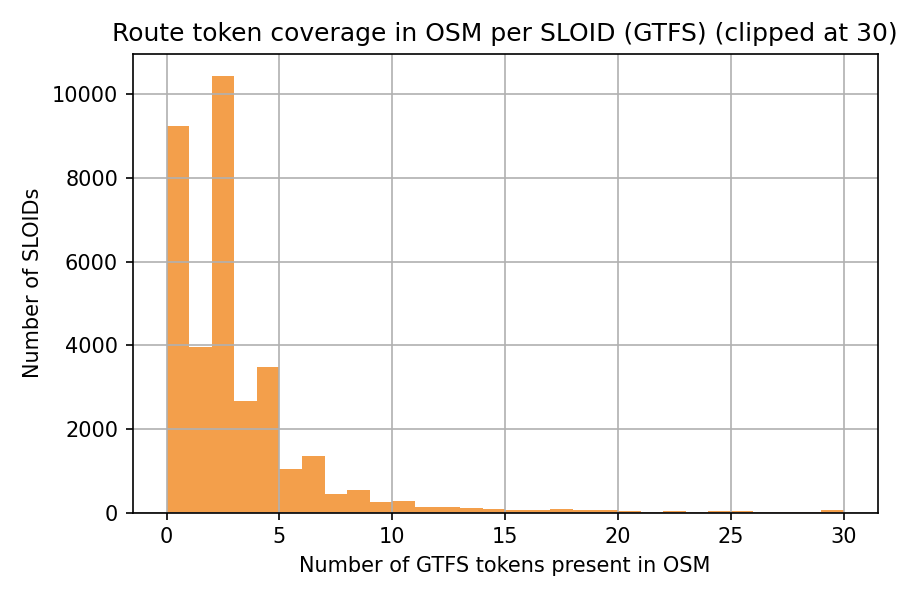
\includegraphics[width=0.75\textwidth]{../figures/chap4/hist_route_token_coverage_per_sloid.png}
  \caption{Nombre de tokens GTFS \((ligne, direction)\) par \texttt{sloid} retrouvés dans OSM (coupée à 30).}
\end{figure}


\section{Bilan et perspectives}

L'appariement par lignes ajoute un signal fort et indépendant qui complète les méthodes exactes, nominales et par distance. L'analyse d'efficacité démontre sa valeur ajoutée substantielle (\textbf{40\%} de nouveaux appariements) tout en maintenant une qualité spatiale élevée (86\% des correspondances sous 25 m).
